\subsection{Aplicación}

Siempre que sea aplicable, la inspiración ha sido tomada de la analogía con la Capa de Negocios. La capa de aplicación se utiliza típicamente para modelar las arquitecturas de los sistemas de información de la empresa, incluida la arquitectura de aplicación que, como se define en el marco del TOGAF, describe la estructura y la interacción de las aplicaciones.

\newpage
\subsubsection{Elementos de la Estructura}
\begin{longtable}{|c|c|c|}
	
	\hline
	Concepto & Descripción & Representación \\ \hline
	
	Componente 
	&
	\begin{tabular}[l]{@{}l@{}}
		Una encapsulación de la funcionalidad\\
		de la aplicación alineada con la \\
		estructura de implementación, que es\\
		modular y reemplazable. Encapsula su\\
		comportamiento y datos, expone los \\
		servicios y los pone a disposición a \\
		través de interfaces.
	\end{tabular}
	& 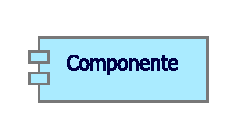
\includegraphics{imgs/aplicacion/componente.pdf}
	\\\hline
	
	Colaboración
	& 
	\begin{tabular}[l]{@{}l@{}}
		Un agregado de dos o más componentes\\
		de la aplicación que trabajan juntos\\
		para realizar un comportamiento de \\
		aplicación colectivo.
	\end{tabular}
	& 
\includegraphics{imgs/aplicacion/colaboracion.pdf}
	\\\hline
	
	Interface
	& 
	\begin{tabular}[l]{@{}l@{}}
		Un punto de acceso donde los servicios\\
		de la aplicación están disponibles para\\
		un usuario, otro componente de la \\
		aplicación o un nodo.
	\end{tabular}
	& 
\includegraphics{imgs/aplicacion/interface.pdf}
	\\\hline
	
	Función
	& 
	\begin{tabular}[l]{@{}l@{}}
		Comportamiento automatizado que puede\\
		realizar un componente de la aplicación.
	\end{tabular}
	& 
\includegraphics{imgs/aplicacion/funcion.pdf}
	\\\hline
	
	Interacción
	& 
	\begin{tabular}[l]{@{}l@{}}
		Una unidad de comportamiento de \\
		aplicación colectiva realizada por \\
		(una colaboración de) dos o más \\
		componentes de la aplicación.
	\end{tabular}
	& 
\includegraphics{imgs/aplicacion/intereaccion.pdf}
	\\\hline
	
	Proceso
	& 
	\begin{tabular}[l]{@{}l@{}}
		Una secuencia de comportamientos de\\
		aplicación que logra un resultado\\
		específico.
	\end{tabular}
	& 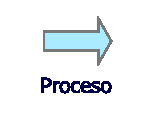
\includegraphics{imgs/aplicacion/proceso.pdf}
	\\\hline
	
	Evento 
	& 
	\begin{tabular}[l]{@{}l@{}}
		Un elemento de comportamiento de la\\
		aplicación que denota un cambio de\\
		estado.
	\end{tabular}
	& 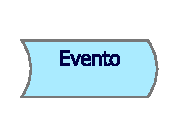
\includegraphics{imgs/aplicacion/evento.pdf}
	\\\hline
	
	Servicio 
	& 
	\begin{tabular}[l]{@{}l@{}}
		Un comportamiento de aplicación \\
		expuesto definido explícitamente.
	\end{tabular}
	& 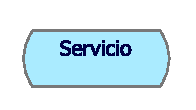
\includegraphics{imgs/aplicacion/servicio.pdf}
	\\\hline
	
	Objeto
	& 
	\begin{tabular}[l]{@{}l@{}}
		Datos estructurados para \\
		procesamiento automatizado.
	\end{tabular}
	& 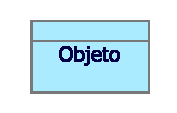
\includegraphics{imgs/aplicacion/objeto.pdf}
	
	
	\\\hline
	\caption{Conceptos: Aplicaciones}
	\label{tab:concepts}
\end{longtable}